\documentclass[a4paper,twoside]{article}
\usepackage[T1]{fontenc}
\usepackage[bahasa]{babel}
\usepackage{graphicx}
\usepackage{graphics}
\usepackage{float}
\usepackage[cm]{fullpage}
\pagestyle{myheadings}
\usepackage{etoolbox}
\usepackage{setspace} 
\usepackage{lipsum} 
\setlength{\headsep}{30pt}
\usepackage[inner=2cm,outer=2.5cm,top=2.5cm,bottom=2cm]{geometry} %margin
\usepackage[plainpages=false,pdfpagelabels,unicode]{hyperref}
\hypersetup{unicode=true,colorlinks=true,linkcolor=blue,citecolor=green,filecolor=magenta,urlcolor=cyan}
% \pagestyle{empty}

\makeatletter
\renewcommand{\@maketitle} {\begin{center} {\LARGE \textbf{ \textsc{\@title}} \par} \bigskip {\large \textbf{\textsc{\@author}} }\end{center} }
\renewcommand{\thispagestyle}[1]{}
\markright{\textbf{\textsc{AIF234002 \textemdash Rencana Kerja Tugas Akhir \textemdash Sem. Ganjil 2025/2026}}}

\newcommand{\HRule}{\rule{\linewidth}{0.4mm}}
\renewcommand{\baselinestretch}{1}
\setlength{\parindent}{0 pt}
\setlength{\parskip}{6 pt}

\onehalfspacing
 
\begin{document}

\title{\@judultopik}
\author{\nama \textendash \@npm} 

%tulis nama dan NPM anda di sini:
\newcommand{\nama}{Ade Rimbo Spencher}
\newcommand{\@npm}{6182001060}
\newcommand{\@judultopik}{Pengembangan Aplikasi Desktop Pemeriksaan Tautan Rusak pada Situs Web} % Judul/topik anda
\newcommand{\jumpemb}{1} % Jumlah pembimbing, 1 atau 2
\newcommand{\tanggal}{25/09/2025}

\maketitle

\pagenumbering{arabic}

\section{Deskripsi}
Situs web merupakan salah satu sarana utama dalam penyebaran informasi dan representasi identitas institusi di era digital. Dalam berbagai sektor, termasuk perguruan tinggi, situs web digunakan sebagai kanal resmi untuk menyampaikan informasi secara luas. Perguruan tinggi memanfaatkan situs web untuk menyediakan beragam konten seperti kalender akademik, pengumuman penting, publikasi ilmiah, dokumentasi kegiatan kampus, serta informasi administratif lainnya. Situs web juga menjadi titik awal interaksi antara institusi dengan calon mahasiswa, mitra kerja, media, dan masyarakat umum.

Pentingnya situs web pada perguruan tinggi juga tercermin dari adanya berbagai sistem pemeringkatan non-akademis yang menjadikan situs web resmi perguruan tinggi sebagai objek penilaian. Dua contoh sistem pemeringkatan tersebut adalah Webometrics dan uniRank. Webometrics\footnote{\url{https://webometrics.info} (Diakses pada 7 April 2025)} merupakan sistem pemeringkatan yang dikembangkan oleh Cybermetrics Lab, sebuah kelompok riset di bawah Consejo Superior de Investigaciones Científicas (CSIC) Spanyol. Sistem ini menilai kehadiran dan visibilitas situs web akademik di internet sebagai cerminan dari kinerja dan dampak institusi dalam ranah digital. Namun, sejak April 2025 laman resmi Webometrics sudah tidak dapat diakses. Sementara itu, uniRank\footnote{\url{https://www.unirank.org/about} (Diakses pada 20 Juli 2025)} adalah sistem pemeringkatan yang berfokus pada popularitas dan kehadiran daring situs web perguruan tinggi. Penilaian pada uniRank dilakukan menggunakan empat metrik independen, yaitu \textit{Majestic Referring Domains} (55\%), \textit{Similarweb Global Rank} (35\%), \textit{Moz Domain Authority} (5\%), dan \textit{Majestic Trust Flow} (5\%). \textit{Majestic Referring Domains} mengukur jumlah domain eksternal unik yang memberikan tautan menuju situs web resmi perguruan tinggi, dengan mempertimbangkan kualitas tautan melalui ambang batas \textit{Trust Flow} tertentu. Sementara itu, \textit{Similarweb Global Rank} mencerminkan tingkat popularitas situs berdasarkan estimasi trafik global yang diterima dari berbagai sumber pengunjung. Berdasarkan kedua sistem tersebut, dapat disimpulkan bahwa visibilitas dan pengalaman pengguna merupakan dua aspek yang penting dari situs web perguruan tinggi dan perlu diperhatikan secara berkelanjutan.



Salah satu tantangan dalam menjaga visibilitas dan pengalaman pengguna dalam mengakses situs web perguruan tinggi adalah keberadaan tautan rusak. Tautan rusak terjadi ketika suatu tautan mengarah ke sumber daya yang sudah tidak tersedia atau tidak dapat diakses, sehingga menghasilkan pesan kesalahan seperti \texttt{404 Not Found} atau \texttt{500 Internal Server Error}. Keberadaan tautan rusak dapat menghambat alur navigasi, menurunkan kepercayaan pengguna terhadap isi situs, serta berdampak negatif terhadap peringkat situs dalam mesin pencari dan sistem pemeringkatan daring, seperti uniRank dan Webometrics. Oleh karena itu, pemantauan dan pemeliharaan tautan secara berkala merupakan langkah penting dalam pengelolaan situs web institusi pendidikan tinggi.


Secara umum, terdapat dua pendekatan dalam memeriksa keberadaan tautan rusak pada situs web, yaitu secara manual dan dengan bantuan perangkat lunak. Pemeriksaan manual menjadi tidak praktis ketika situs memiliki ratusan bahkan ribuan halaman. Untuk mengatasi hal ini, tersedia berbagai layanan daring seperti Broken Link Checker\footnote{\url{https://www.brokenlinkcheck.com/} (Diakses pada 20 Juli 2025)}. Broken Link Checker merupakan alat berbasis web yang secara otomatis memindai halaman-halaman dalam sebuah situs web dan mendeteksi tautan rusak di dalamnya.

Gambar~\ref{fig:gambar-contoh-brokenlinkcheck} menunjukkan hasil pemindaian pada situs web Informatika UNPAR menggunakan layanan Broken Link Checker, di mana terdeteksi beberapa tautan rusak yang tersebar di berbagai halaman. Dalam laporannya, Broken Link Checker menampilkan informasi penting seperti URL dari tautan rusak yang ditemukan, teks yang menjadi jangkar (\textit{anchor text}) dari tautan tersebut, halaman tempat tautan itu ditemukan, serta respons dari server dalam bentuk kode status HTTP seperti \texttt{404} atau \texttt{500}. Layanan ini juga menyediakan tautan langsung menuju bagian kode sumber tautan rusak ditemukan untuk mempermudah pelacakan lokasi tautan rusak dalam dokumen HTML.

\begin{figure}[H]
    \centering
    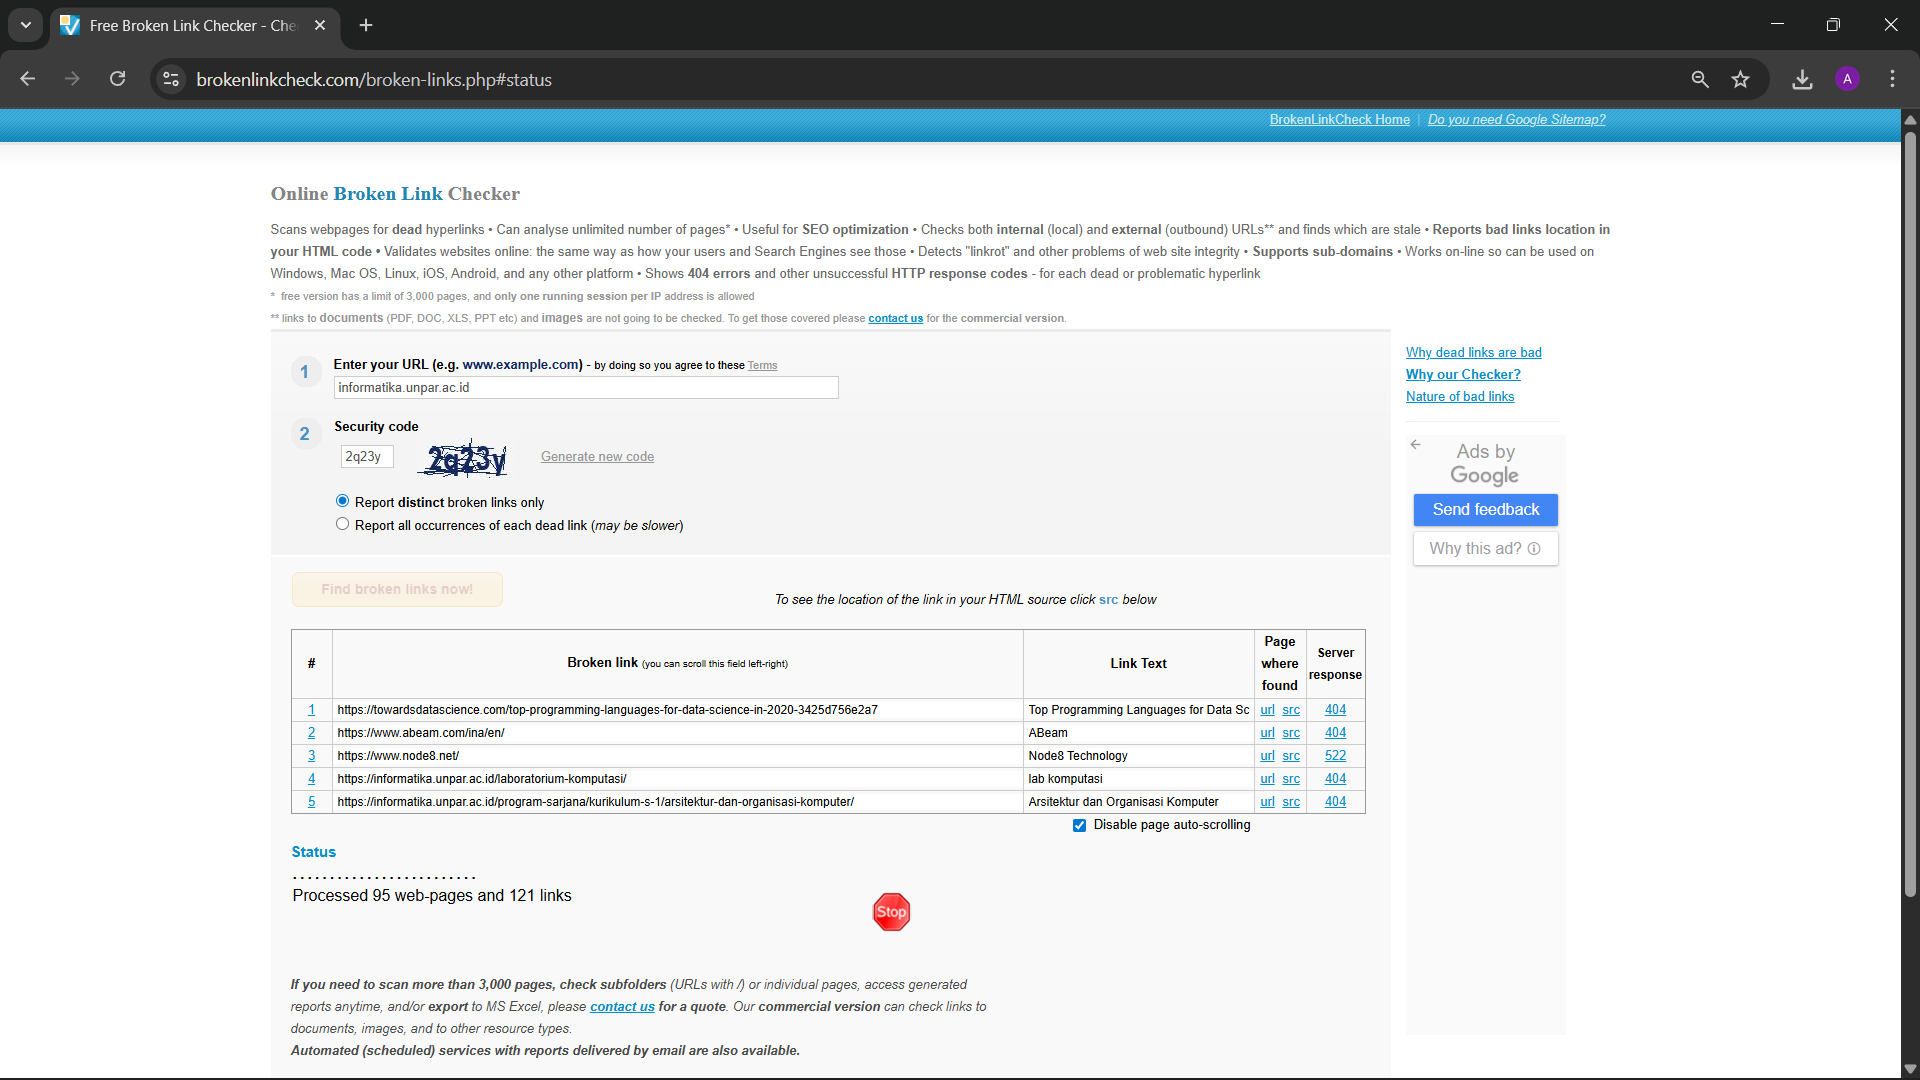
\includegraphics[width=0.85\textwidth]{broken-link-checker.png}
    \caption{Tampilan Broken Link Checker}
    \label{fig:gambar-contoh-brokenlinkcheck}
\end{figure}


Dalam penelitian ini akan dikembangkan sebuah perangkat lunak berbasis desktop yang dapat digunakan untuk memeriksa keberadaan tautan rusak pada situs web secara otomatis. Perangkat lunak ini akan menerima masukan berupa URL alamat situs web, kemudian menelusuri halaman-halaman yang saling terhubung di dalamnya untuk mengidentifikasi seluruh tautan yang terdapat pada situs tersebut. Selanjutnya, setiap tautan akan diperiksa dan dievaluasi respons yang diberikan oleh server. Berdasarkan hasil pemeriksaan tersebut, perangkat lunak akan menghasilkan laporan yang memuat informasi mengenai tautan-tautan yang terdeteksi rusak. Untuk mempermudah pengguna dalam menjalankan proses pemeriksaan dan membaca hasilnya, perangkat lunak ini akan dilengkapi dengan antarmuka pengguna grafis yang intuitif.

\vspace{5pt}

\section{Rumusan Masalah}
Rumusan masalah dari penelitian ini adalah sebagai berikut:
\begin{enumerate}
    \setlength\itemsep{1pt}

    \item Bagaimana mengembangkan perangkat lunak berbasis desktop yang dapat melakukan pemeriksaan tautan rusak pada situs web?
    
    \item Bagaimana melakukan pengujian perangkat lunak pemeriksa tautan rusak dan membandingkan hasil yang diperoleh dengan perangkat lunak serupa?
    
\end{enumerate}


\section{Tujuan}
Tujuan dari penelitian ini adalah sebagai berikut:

\begin{enumerate}

    \item Mengembangkan perangkat lunak berbasis desktop yang mampu melakukan pemeriksaan terhadap tautan rusak pada situs web.
    
    \item Melakukan pengujian terhadap perangkat lunak pemeriksa tautan rusak yang dikembangkan, serta membandingkan hasilnya dengan perangkat lunak serupa.
    
\end{enumerate}

\section{Deskripsi Perangkat Lunak}
Perangkat lunak yang akan dikembangkan dalam tugas akhir ini adalah sebuah aplikasi desktop bernama \textit{Broken Link Checker}. Aplikasi ini dirancang untuk membantu pengguna dalam memeriksa keberadaan tautan rusak pada sebuah situs web, dengan fitur utama sebagai berikut:

\begin{itemize}
    
    \item Pengguna dapat memasukkan sebuah URL awal (\textit{seed URL}) sebagai titik awal pemeriksaan.
    
    \item Aplikasi akan melakukan \textit{web crawling} dengan pendekatan \textit{Breadth-First Search} (BFS) terhadap halaman-halaman yang berada dalam satu \textit{host} yang sama dan mengekstrak seluruh tautan yang ditemukan pada setiap halaman.
    
    \item Setiap tautan yang ditemukan akan diperiksa, apabila tautan tidak dapat diakses atau menggembalikan HTTP \textit{status code} yang lebih besar dari 400, maka akan ditandai sebagai tautan rusak.
    
    \item Hasil pemeriksaan akan ditampilkan melalui antarmuka pengguna grafis secara \textit{streaming}, dengan pemisahan antara tabel halaman yang berhasil di-\textit{crawling} dan tabel tautan rusak.
    
    \item Aplikasi menyediakan fitur ekspor hasil pemeriksaan tautan rusak dalam format Excel untuk memudahkan analisis dan dokumentasi lebih lanjut.
    
    \item Proses pemeriksaan dilengkapi dengan mekanisme sebagai berikut:
    \begin{itemize}
        
        \item \textit{Timeout}: membatasi waktu tunggu maksimum pada setiap permintaan HTTP, sehingga aplikasi tidak terjebak menunggu respons server yang lambat atau tidak merespons.
        
        \item \textit{Retry}: mengulangi kembali permintaan yang gagal dalam kondisi tertentu dengan jumlah percobaan terbatas.
        
        \item \textit{rate limiting}: mengendalikan frekuensi permintaan agar tidak membebani server tujuan dan mencegah perangkat lunak dianggap sebagai serangan.
    \end{itemize}
\end{itemize}

\section{Detail Pengerjaan Tugas Akhir}
Bagian-bagian pekerjaan yang akan dilakukan dalam pengerjaan tugas akhir ini adalah sebagai berikut:

\begin{enumerate}
    
    \item Melakukan studi literatur terhadap protokol HTTP, URI, situs web, dan \textit{web crawling}.
    
    \item Melakukan studi literatur dan eksperimen terhadap teknologi yang akan digunakan, yaitu Jsoup, Java \texttt{HttpClient}, dan JavaFX.
    
    \item Melakukan analisis terhadap permasalahan pemeriksaan tautan rusak pada situs web, meninjau perangkat lunak serupa, serta merumuskan kebutuhan fungsional dan non-fungsional perangkat lunak.
    
    \item Melakukan perancangan kelas, perancangan alur dan perancangan antarmuka pengguna perangkat lunak.
    
    \item Mengimplementasikan perangkat lunak berdasarkan perancangan yang telah dibuat.
    
    \item Melakukan pengujian fungsional dan eksperimental serta dilakukan analisis terhadap hasil pengujian.
    
    \item Menulis dokumen tugas akhir.
\end{enumerate}


\section{Rencana Kerja}
Rincian capaian yang akan diselesaikan di Tugas Akhir 2 adalah sebagai berikut:

\begin{enumerate}
    
    \item Melakukan studi literatur terhadap protokol HTTP, URI, situs web, dan \textit{web crawling}.
    
    \item Melakukan studi literatur dan eksperimen terhadap teknologi yang akan digunakan, yaitu Jsoup, Java \texttt{HttpClient}, dan JavaFX.
    
    \item Melakukan analisis terhadap permasalahan pemeriksaan tautan rusak pada situs web, meninjau perangkat lunak serupa, serta merumuskan kebutuhan fungsional dan non-fungsional perangkat lunak.
    
    \item Melakukan perancangan kelas, perancangan alur dan perancangan antarmuka pengguna perangkat lunak.
    
    \item Mengimplementasikan perangkat lunak berdasarkan perancangan yang telah dibuat.
    
    \item Melakukan pengujian fungsional dan eksperimental serta dilakukan analisis terhadap hasil pengujian.
    
    \item Menulis dokumen tugas akhir.
\end{enumerate}

\vspace{1cm}
\centering Bandung, \tanggal\\
\vspace{2cm} \nama \\ 
\vspace{1cm}

Menyetujui, \\
\ifdefstring{\jumpemb}{2}{
\vspace{1.5cm}
\begin{centering} Menyetujui,\\ \end{centering} \vspace{0.75cm}
\begin{minipage}[b]{0.45\linewidth}
% \centering Bandung, \makebox[0.5cm]{\hrulefill}/\makebox[0.5cm]{\hrulefill}/2013 \\
\vspace{2cm} Nama: \makebox[3cm]{\hrulefill}\\ Pembimbing Utama
\end{minipage} \hspace{0.5cm}
\begin{minipage}[b]{0.45\linewidth}
% \centering Bandung, \makebox[0.5cm]{\hrulefill}/\makebox[0.5cm]{\hrulefill}/2013\\
\vspace{2cm} Nama: \makebox[3cm]{\hrulefill}\\ Pembimbing Pendamping
\end{minipage}
\vspace{0.5cm}
}{
% \centering Bandung, \makebox[0.5cm]{\hrulefill}/\makebox[0.5cm]{\hrulefill}/2013\\
\vspace{2cm} Pascal Alfadian Nugroho, M.Comp\\ Pembimbing Tunggal
}
\end{document}